\documentclass[nooutcomes, handout]{ximera}
%% handout
%% space
%% newpage
%% numbers
%% nooutcomes

%I added the commands here so that I would't have to keep looking them up
\newcommand{\RR}{\mathbb R}
\renewcommand{\d}{\,d}
\newcommand{\dd}[2][]{\frac{d #1}{d #2}}
\renewcommand{\l}{\ell}
\newcommand{\ddx}{\frac{d}{dx}}
\everymath{\displaystyle}
\newcommand{\dfn}{\textbf}
\newcommand{\eval}[1]{\bigg[ #1 \bigg]}



% \newcommand{\RR}{\mathbb R}
\renewcommand{\d}{\,d}
\newcommand{\dd}[2][]{\frac{d #1}{d #2}}
\renewcommand{\l}{\ell}
\newcommand{\ddx}{\frac{d}{dx}}
\newcommand{\dfn}{\textbf}
\newcommand{\eval}[1]{\bigg[ #1 \bigg]}

\usepackage{multicol}

\renewenvironment{freeResponse}{
\ifhandout\setbox0\vbox\bgroup\else
\begin{trivlist}\item[\hskip \labelsep\bfseries Solution:\hspace{2ex}]
\fi}
{\ifhandout\egroup\else
\end{trivlist}
\fi} %% we can turn off input when making a master document

\title{Recitation 29}  

\begin{document}
\begin{abstract}		\end{abstract}
\maketitle

\section{Substitution Rule Part II }
% \begin{problem}[warmup]
%   What are two substitutions that can be used to evaluate the integral
%   \begin{equation*}
%     \int x \sqrt{x+8} \d x
%   \end{equation*}
	
% 		\begin{freeResponse}
%                   Two substitutions which work are $u=x+8$ and
%                   $v=\sqrt{x+8}$.  I find the $u=x+8$ to be the more
%                   ``obvious" solution, so let us work through that one
%                   first.
%                   \begin{equation*}
%                     u=x+8 \quad \Longrightarrow \quad \d u = \d x \quad \text{and} \quad x = u-8
%                   \end{equation*}
%                   Substituting into the original integral and solving:
%                   \begin{align*}
%                     \int x \sqrt{x+8} \d x &= \int (u-8) \sqrt{u} \d u  \\
%                                            &= \int (u^{\frac{3}{2}} - 8u^{\frac{1}{2}} ) \d u  \\
%                                            &= \frac{2}{5} u^{\frac{5}{2}} - 8 \cdot \frac{2}{3} u^{\frac{3}{2}} + C  \\
%                                            &= \frac{2}{5} (x+8)^{\frac{5}{2}} - \frac{16}{3} (x+8)^{\frac{3}{2}} + C
%                   \end{align*}
		
%                   To the other solution, letting $v=\sqrt{x+8}$ gives:
%                   \begin{equation*}
%                     \d v = \frac{1}{2 \sqrt{x+8}} \d x = \frac{1}{2v} \d x 	\quad	\Longrightarrow \quad \d x = 2v \d v
%                   \end{equation*}
%                   and
%                   \begin{equation*}
%                     v = \sqrt{x+8} \quad \Longrightarrow \quad v^2 = x+8 \quad \Longrightarrow \quad x= v^2-8
%                   \end{equation*}
%                   Substituting into the original integral and solving:
%                   \begin{align*}
%                     \int x \sqrt{x+8} \d x &= \int (v^2-8)(v)(2v)\d v  \\
%                                            &= \int (2v^4 - 16v^2) \d v  \\
%                                            &= \frac{2}{5} v^5 - \frac{16}{3} v^3 + C  \\
%                                            &= \frac{2}{5} (\sqrt{x+8})^5 - \frac{16}{3} (\sqrt{x+8})^3 + C
%                   \end{align*}
		
% 		\end{freeResponse}
%               \end{problem}

%problem 2
% \begin{problem}
% Compute the  integral

% 	% \item  $\int \cos(x) \sqrt{\sin(x)} \d x$
% 	% 	\begin{freeResponse}
% 	% 	Let $v = \sin(x)$.  Then $\d v = \cos(x) \d x$, and so
% 	% 		\begin{align*}
% 	% 		\int \cos(x) \sqrt{\sin(x)} \d x &= \int \sqrt{v} \d v  \\
% 	% 		&= \frac{2}{3} v^{\frac{3}{2}} + C  \\
% 	% 		&= \frac{2}{3} (\sin(x))^{\frac{3}{2}} + C.
% 	% 		\end{align*}
% 	% 	\end{freeResponse}
		



	
% 	%part a
		
		
% 	% %part b
% 	 $\int \left( 3t^2 - 4 + \frac{1}{t} \right) e^{t^3 - 4t + \ln(t) - 9} \d t$
% 		\begin{freeResponse}
% 		This problem looks a lot more difficult than it really is.  Let $w=t^3 - 4t + \ln(t) - 9$.  
% 		Then $\d w = \left( 3t^2 - 4 + \frac{1}{t} \right) \d t$.  But this is exactly the coefficient of the exponential term in the integral.  So
% 			\begin{align*}
% 			\int \left( 3t^2 - 4 + \frac{1}{t} \right) e^{t^3 - 4t + \ln(t) - 9} \d t &= \int e^w \d w  \\
% 			&= e^w + C  \\
% 			&= e^{t^3 - 4t + \ln(t) - 9} + C.
% 			\end{align*}
% 		\end{freeResponse}
		
% \end{problem}
	
%problem 4
\begin{problem}
  \mbox{}
  \begin{itemize}
  \item Part of this recitation's focus is on performing the
    substitution rule for definite integrals. The other part focuses
    on the connection between velocity, net area, displacement, and
    distance.

    \item For problem 1 only pick one to work on.

    \item For problem 2 only pick one to work on.

    \item For problem 3 sketch the graph of the integrand over the
      interval $[-2,2]$ to help illustrate why we can't perform the
      substitution over this interval.

    \item After solving problem 5 I also recommend graphing both
      velocity $v$ and speed $|v|$. The graph for speed (as well as
      the sign chart for $v$) is helpful in motivating decomposing a
      definite integral when the integrand is the absolute value of a
      function.
  \end{itemize}

Evaluate the following integrals:

	\begin{enumerate}
	
	%part a
	\item  $\int_{-2}^1 t^2 \sin(t^3) \d t$
		\begin{freeResponse}
		Let $u=u(t) = t^3$, where $``u(t)"$ is just meant to indicate that the variable $u$ is really a function of $t$.  Then $\d u = 3t^2 \d t$.  But also notice that
			\begin{align*}
			u(-2) &= (-2)^3 = -8  \\
			u(1) &= 1^3 = 1
			\end{align*}
		Then
			\begin{align*}
			\int_{-2}^1 t^2 \sin(t^3) \d t &= \frac{1}{3} \int_{-2}^1 3 t^2 \sin(t^3) \d t  \\
			&= \frac{1}{3} \int_{-8}^1 \sin(u) \d u  \\
			&= - \frac{1}{3} \eval{\cos(u)}_{-8}^1  \\
			&= - \frac{1}{3} ( \cos(1) - \cos(-8)).
			\end{align*}
		\end{freeResponse}
		
		
		
	%part b
	\item  $\int_0^{\frac{1}{2}} \frac{13e^x}{3e^x - 5} \d x$
		\begin{freeResponse}
		Let $v=3e^x - 5$.  Then
			\begin{align*}
			&\d v = 3e^x \d x  \\
			&v(0) = 3e^0 -5= 3-5=-2  \\
			&v\left( \frac{1}{2} \right) = 3e^{\frac{1}{2}} - 5.
			\end{align*}
		So
			\begin{align*}
			\int_0^{\frac{1}{2}} \frac{13e^x}{3e^x - 5} \d x &= \frac{13}{3} \int_0^{\frac{1}{2}} \frac{3e^x}{3e^x - 5} \d x  \\
			&= \frac{13}{3} \int_{-2}^{3e^{\frac{1}{2}}-5} \frac{1}{v} \d v  \\
			&= \frac{13}{3} \eval{\ln|v|}_{-2}^{3e^{\frac{1}{2}}-5}  \\
			&= \frac{13}{3} \left( \ln|3e^{\frac{1}{2}}-5| - \ln|-2| \right).  \\
			\end{align*}
		\end{freeResponse}
		
		
		
	\end{enumerate}
			
			
	
\end{problem}

\begin{problem}
Evaluate the following integrals:

	\begin{enumerate}
	
	%part a
	\item  $\int_1^4 \frac{e^{\sqrt{x}}}{3\sqrt{x}} \d x$
		\begin{freeResponse}
		Let $w=\sqrt{x}$.  Then
			\begin{align*}
			&\d w = \frac{1}{2 \sqrt{x}} \d x  \\
			&w(1) = \sqrt{1} = 1  \\
			&w(4) = \sqrt{4} = 2.
			\end{align*}
		So
			\begin{align*}
			\int_1^4 \frac{e^{\sqrt{x}}}{3\sqrt{x}} \d x &= \frac{2}{3} \int_1^4 \frac{e^{\sqrt{x}}}{2\sqrt{x}} \d x  \\
			&= \frac{2}{3} \int_1^2 e^w \d w  \\
			&= \frac{2}{3} \eval{e^w}_1^2  \\
			&= \frac{2}{3} (e^2 - e).
			\end{align*}
		\end{freeResponse}
		
		
		
	%part b
	\item  $\int_{\frac{\pi}{3}}^{\frac{\pi}{2}} \sin(x) \sec^2(\cos(x)) \d x$
		\begin{freeResponse}
		Let $u=\cos(x)$.  Then
			\begin{align*}
			&\d u = -\sin(x) \d x  \\
			&u\left( \frac{\pi}{3} \right) = \frac{1}{2}  \\
			&u\left( \frac{\pi}{2} \right) = 0.
			\end{align*}
		So
			\begin{align*}
			\int_{\frac{\pi}{3}}^{\frac{\pi}{2}} \sin(x) \sec^2(\cos(x)) \d x &= - \int_{\frac{1}{2}}^0 \sec^2(u) \d u   \\
			&= - \eval{\tan(u)}_{\frac{1}{2}}^0  \\
			&=  -\left( 0 - \tan\left( \frac{1}{2} \right) \right)  \\
			&= \tan \left( \frac{1}{2} \right).
			\end{align*}
		\end{freeResponse}
		
		
		
	\end{enumerate}
			
			
	
\end{problem}















%problem 1
% \begin{problem}
% Compute the integral


	
% 	% %part a
% 	% \item  $\int 2t \sin \left( t^2 \right) \d t$
% 	% 	\begin{freeResponse}
% 	% 	Let $w=t^2$.  Then $\d w = 2t \d t$, and so
% 	% 		\begin{align*}
% 	% 		\int 2t \sin(t^2) \d t &= \int \sin(w) \d w  \\
% 	% 		&= - \cos(w) + C  \\
% 	% 		&= - \cos(t^2) + C.
% 	% 		\end{align*}
% 	% 	\end{freeResponse}
		
		
		
% 	%part b
% 	  $\int \sec^2(x) \tan(x) \d x$
% 		\begin{freeResponse}
% 		Let $u = \tan(x)$.  Then $\d u = \sec^2 (x) \d x$, and so
% 			\begin{align*}
% 			\int \sec^2(x) \tan(x) \d x &= \int u \d u  \\
% 			&= \frac{1}{2} u^2 + C  \\
% 			&= \frac{1}{2} \tan^2(x) + C.
% 			\end{align*}
% 		Note that the substitution $v=\sec(x)$ would also work to solve this problem.  
% 		It is a good exercise to work this out!
% 		\end{freeResponse}
% \end{problem}







%problem 3
% \begin{problem}
% Compute the integral

% 	% %part a
% 	%   $\int \frac{x^2 }{1 + x^2} \d x$
% 	% 	\begin{freeResponse}
% 	% 	In general, when integrating a rational function where the degree of the numerator is greater than or equal to the degree
% 	% 	of the denominator, you want to do long division to get the smallest possible degree in the numerator.  
% 	% 	But watch this slick little trick:
% 	% 		\begin{equation*}
% 	% 		\frac{x^2}{1+x^2} = \frac{1 + x^2 - 1}{1+x^2} = \frac{1+x^2}{1+x^2} - \frac{1}{1+x^2} = 1 - \frac{1}{1+x^2}.
% 	% 		\end{equation*}
% 	% 	So
% 	% 		\begin{align*}
% 	% 		\int \frac{x^2 }{1 + x^2} \d x &= \int \left( 1 - \frac{1}{1+x^2} \right) \d x  \\
% 	% 		&= x - \arctan(x) + C.
% 	% 		\end{align*}
% 	% 	I learned the trick above through tons and tons of practice solving integrals.  
% 	% 	So guess what is a good idea for you to do before the final exam???
% 	% 	\end{freeResponse}
		
		
		
% 	%part b
% 	  $ \int \frac{1+3x}{4+4x^2} \d x$
% 		\begin{freeResponse}
% 		First notice that
% 			\begin{equation*}
% 			\int \frac{1+3x}{4+4x^2} \d x = \frac{1}{4} \int \frac{1+3x}{1+x^2} \d x = \frac{1}{4} \int \left( \frac{1}{1+x^2} + \frac{3x}{1+x^2} \right) \d x.
% 			\end{equation*}
% 		The first integral is $\arctan(x)$, and so we have
% 			\begin{equation}\label{3b1}
% 			\int \frac{1+3x}{4+4x^2} \d x = \frac{1}{4} \arctan(x) + \frac{3}{4} \int \frac{x}{1+x^2} \d x.
% 			\end{equation}
% 		We can solve this second integral by substitution.  Let $u=1+x^2$.  Then $\d u = 2x \d x$ and $\frac{1}{2} \d u = x \d x$.  So
% 			\begin{equation}\label{3b2}
% 			\int \frac{x}{1+x^2} \d x = \frac{1}{2} \int \frac{1}{u} \d u = \frac{1}{2} \ln|u| +C = \frac{1}{2} \ln(1+x^2) + C.
% 			\end{equation}
% 		Plugging equation \eqref{3b2} into equation \eqref{3b1} yields
% 			\begin{equation*}
% 			\int \frac{1+3x}{4+4x^2} \d x = \frac{1}{4} \arctan(x) + \frac{3}{8} \ln(1+x^2) + C.
% 			\end{equation*}
% 		\end{freeResponse}
		
		
		
	
			
			
		
% \end{problem}







%problem 6
%\begin{problem}
% Evaluate the following integrals:

% 	\begin{enumerate}
	
% 	%part a
% 	\item  $\int \frac{13x^7}{\sqrt{3x^4-5}} \d x$
% 		\begin{freeResponse}
% 		Let $v = 3x^4 - 5$.  Then
% 			\begin{align*}
% 			&\d v = 12 x^3 \d x  \\
% 			&x^4 = \frac{1}{3} (v + 5).
% 			\end{align*}
% 		So
% 			\begin{align*}
% 			\int \frac{13x^7}{\sqrt{3x^4-5}} \d x &= \frac{13}{12} \int \frac{(x^4)(12 x^3)}{\sqrt{3x^4-5}} \d x  \\
% 			&= \frac{13}{12} \int \frac{\frac{1}{3} (v+5)}{\sqrt{v}} \d v  \\
% 			&= \frac{13}{36} \int \left( v^{\frac{1}{2}} + 5v^{-\frac{1}{2}} \right) \d v  \\
% 			&= \frac{13}{36} \left( \frac{2}{3} v^{\frac{3}{2}} + 10 v^{\frac{1}{2}} \right) + C  \\
% 			&= \frac{13}{54} (3x^4-5)^{\frac{3}{2}} + \frac{65}{18} \sqrt{3x^4 - 5} + C.
% 			\end{align*}
% 		\end{freeResponse}
		
		
		
% 	%part b
% 	\item  $\int \frac{x^3}{x^2 - 3} \d x$
% 		\begin{freeResponse}
% 		Let $w = x^2 - 3$.  Then
% 			\begin{align*}
% 			&\d w = 2x \d x  \\
% 			&x^2 = w + 3.
% 			\end{align*}
% 		So
% 			\begin{align*}
% 			\int \frac{x^3}{x^2 - 3} \d x &= \frac{1}{2} \int \frac{(x^2)(2x)}{x^2 - 3} \d x  \\
% 			&= \frac{1}{2} \int \frac{w+3}{w} \d w  \\
% 			&= \frac{1}{2} \int \left(1 + \frac{3}{w} \right) \d w  \\
% 			&= \frac{1}{2} \left( w + 3 \ln|w| \right) + C  \\
% 			&= \frac{1}{2} \left( x^2 - 3 + 3\ln|x^2-3| \right) + C.
% 			\end{align*}
% 		\end{freeResponse}
		
		
		
% 	\end{enumerate}
			
			
	
% \end{problem}



\newpage



%problem 7
\begin{problem}
Find the error in the following ``solution":

Find $\int_{-2}^2 \frac{1}{x^8 - 1} \d x$

	\begin{image}
	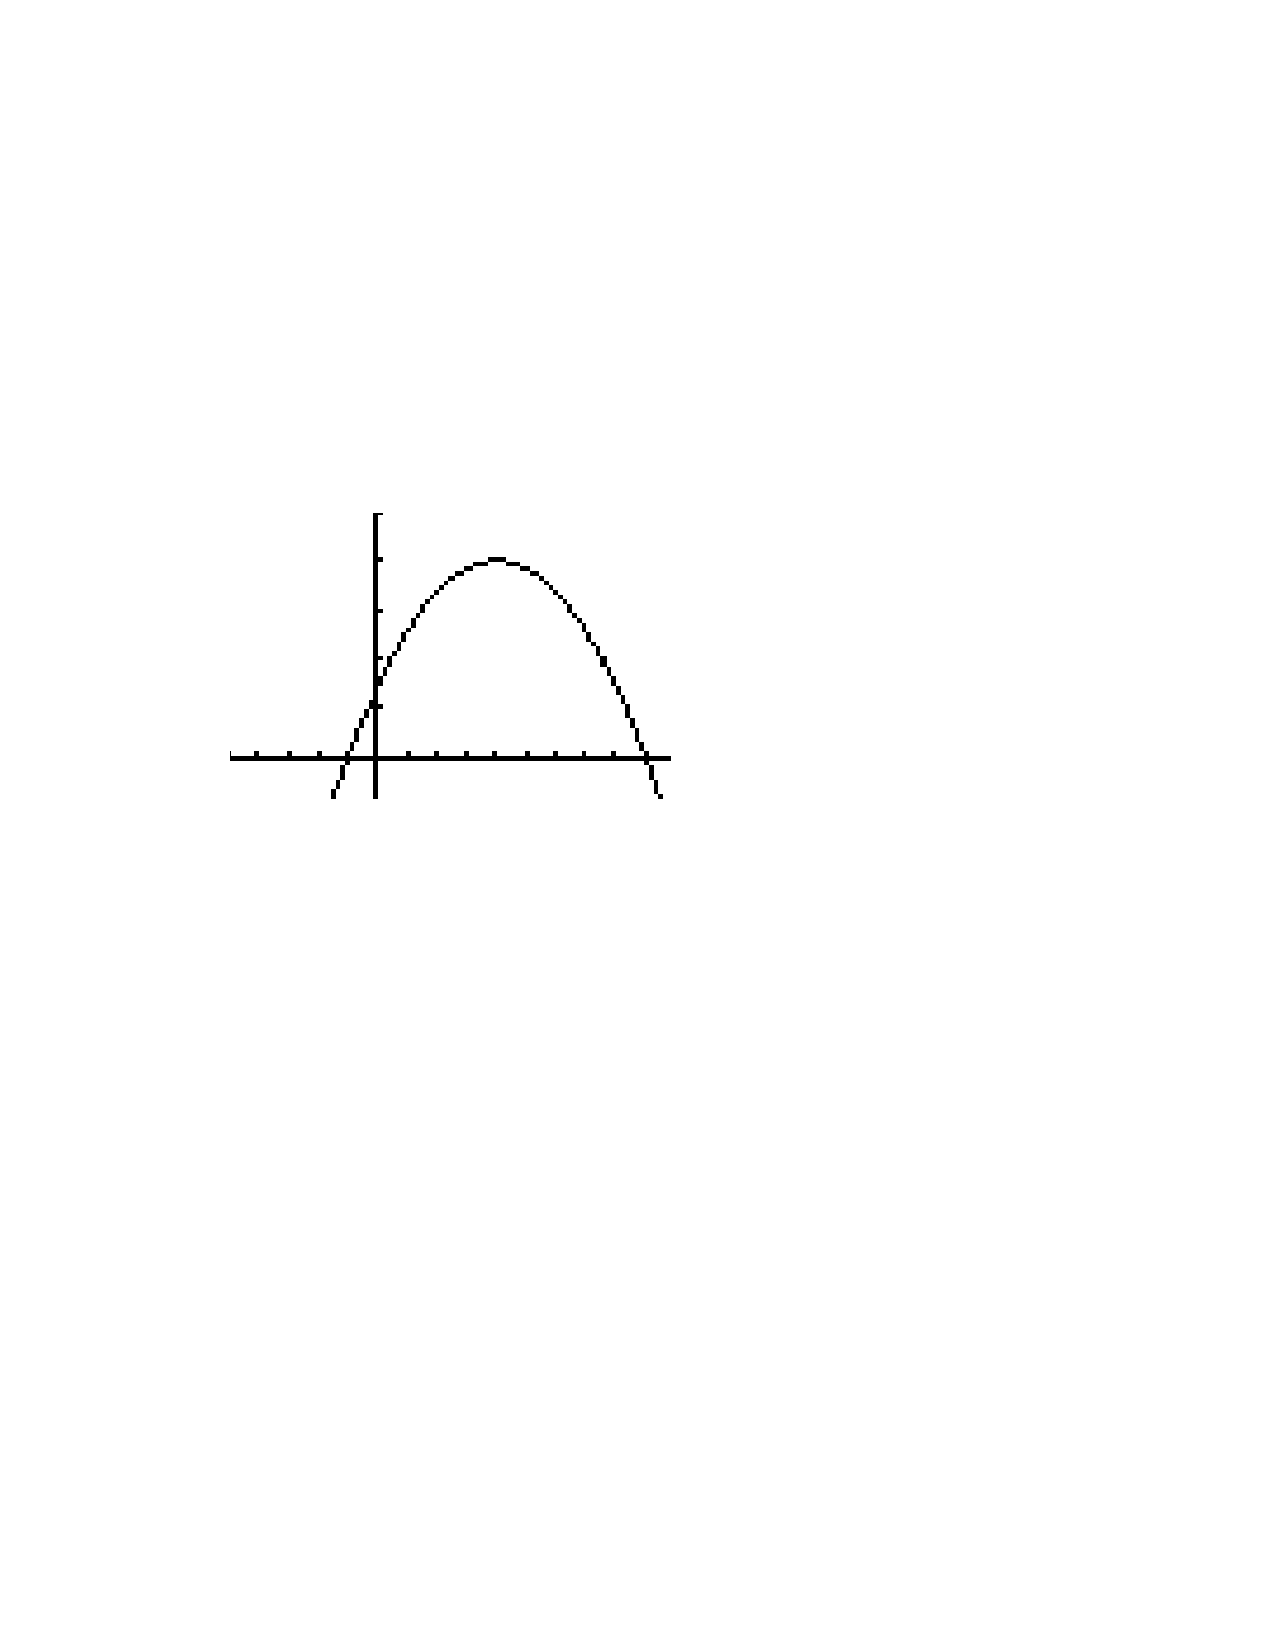
\includegraphics[trim= 120 320 350 180]{Figure1.pdf}
	\end{image}

	\begin{freeResponse}
	The error is that the function $\frac{1}{x^8-1}$ is not defined at $x=1$, and is therefore not continuous on the interval $[-2,2]$.
	\end{freeResponse}
\end{problem}

\section{Velocity and Net Change}

\begin{problem}
  If the velocity of an object moving along a straight line is
  positive, does the displacement of the object equal the distance the
  object traveled?  Why or why not?
  \begin{freeResponse}
    Yes, if the velocity is positive then $\left| v(t) \right|=v(t)$.
    Then (informally)
    \begin{equation*}
      \text{displacement } = \int_a^b v(t) \d t = \int_a^b \left| v(t) \right| \d t = \text{ distance traveled}.
    \end{equation*}
  \end{freeResponse}
\end{problem}





\begin{problem}
Solve the following word problems:

	\begin{enumerate}
	
	%part a
	\item  The velocity function for a man walking along a straight road which runs east and west is given by 
	$v(t) = -t^2 + 4t - 3$ feet per minute.
		
		\begin{enumerate}
		
		%part ai
		\item[i.]  Find the total displacement the man traveled from $2$ minutes to $6$ minutes (assume east is positive). 
			\begin{freeResponse}
			The man's total displacement is given by $\int_2^6 v(t) \d t$.  So we compute:
				\begin{align*}
				\int_2^6 v(t) \d t &= \int_2^6 (-t^2 + 4t - 3) \d t  \\
				&= \eval{- \frac{1}{3} t^3 + 2t^2 - 3t}_2^6  \\
				&= (-72 + 72 - 18) - \left( - \frac{8}{3} + 8 - 6 \right)  \\
				&= \frac{8}{3} - 20 = - \frac{52}{3}.
				\end{align*}
			So the man's displacement is $\frac{52}{3}$ feet west of his original location.
			\end{freeResponse}
				
		%part aii
		\item[ii.]  Find the total distance the man traveled from $2$ minutes to $6$ minutes. 
			\begin{freeResponse}
			First notice that $v(t) = -(t^2 - 4t + 3) = -(t-1)(t-3)$.  So we can see that
				\begin{align*}
				v(t) &> 0 \text{ when }  2 \leq t < 3.  \\
				v(t) &< 0 \text{ when } 3 < t \leq 6.
				\end{align*}
			Thus, the total distance that the man traveled from $2$ minutes to $6$ minutes is:
				\begin{align*}
				\int_2^6 \left| v(t) \right| \d t &= \int_2^3 \left| v(t) \right| \d t + \int_3^6 \left| v(t) \right| \d t  \\
				&= \int_2^3 v(t) \d t + \int_3^6 - v(t) \d t  \\
				&= \int_2^3 (-t^2 + 4t - 3) \d t - \int_3^6 (-t^2 + 4t - 3) \d t  \\
				&= \eval{- \frac{1}{3} t^3 + 2t^2 - 3t}_2^3 - \eval{- \frac{1}{3} t^3 + 2t^2 - 3t}_3^6  \\
				&= \left( (-9+18-9) - (- \frac{8}{3} + 8 - 6) \right) -  \\
				& \left( (-72+72-18)-(-9+18-9) \right)  \\
				&= \left(0 - 2 + \frac{8}{3} \right) - \left( -18 - 0 \right)  \\
				&=  16 + \frac{8}{3} = \frac{56}{3}.
				\end{align*}
			So, the total distance that the man traveled is $\frac{56}{3}$ feet.
			\end{freeResponse}
				
		%part aiii
		\item[iii.]  Suppose that the man's position $2$ minutes into the trip is $5$ feet east of his mailbox.  What is his position (relative to his mailbox) at $6$ minutes.
			\begin{freeResponse}
			$s(6) = s(0) + \int_2^6 v(t) \d t = 5 + \left(- \frac{52}{3} \right) = - \frac{37}{3}. $
			
			So the man's position at $6$ minutes is $\frac{37}{3}$ feet west of his mailbox.
			\end{freeResponse}
				
		\end{enumerate}
		
		
		
	%part b
	\item  Sammy the Snail sets up camp in the median of I-70 and, starting at noon and ending at 6pm, hikes back and forth along the highway.  He starts his hike at his campsite.  His velocity at time $t$ hours (after noon)  is given by $v(t)=(t-2)(t-5)$ inches per hour.  Find the total distance Sammy travelled on his hike.  
		\begin{freeResponse}
		The total distance that Sammy travels is $\int_0^6 \left| v(t) \right| \d t$.  
		The following picture indicates where $v(t)$ is positive and negative:
			\begin{image}
			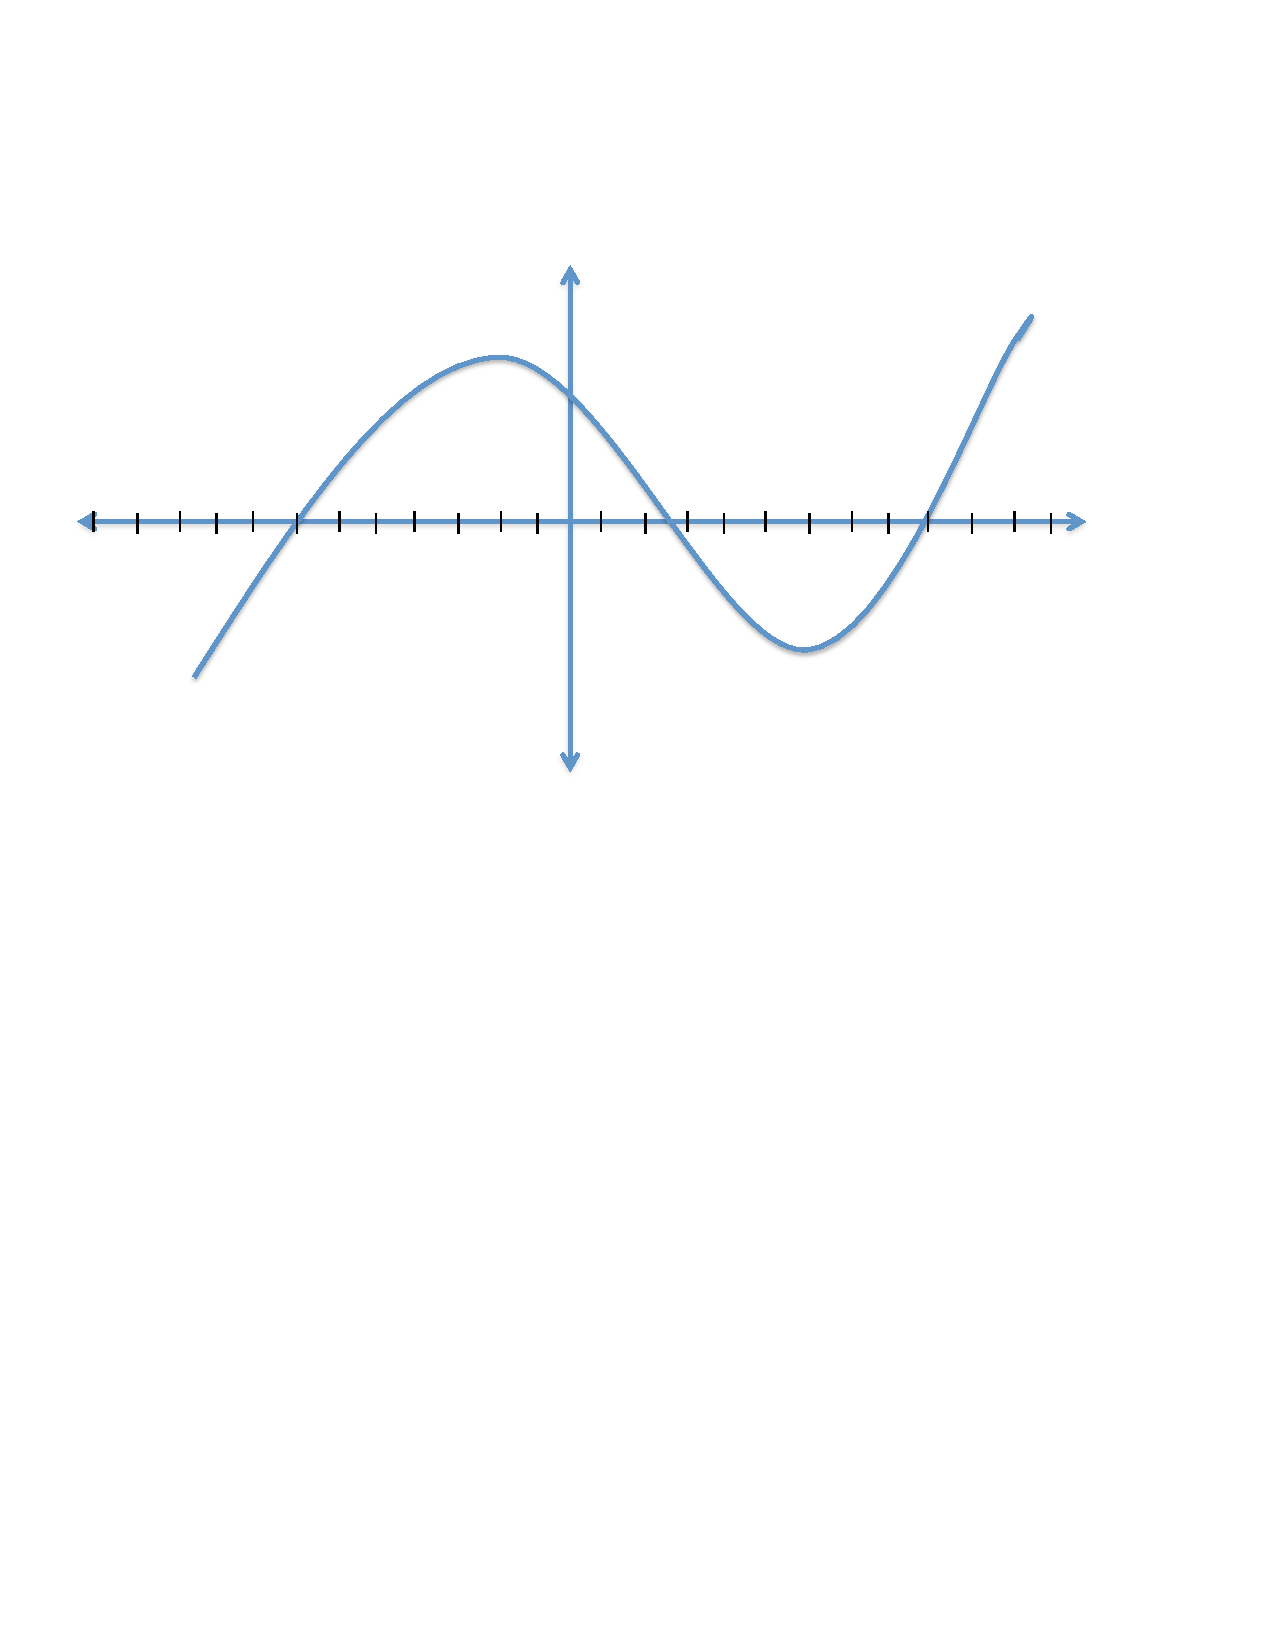
\includegraphics[trim= 170 400 250 290]{Figure2.pdf}
			\end{image}
		So we compute:
			\begin{align*}
			\int_0^6 \left| v(t) \right| \d t &= \int_0^2 \left| v(t) \right| \d t + \int_2^5 \left| v(t) \right| \d t + \int_5^6 \left| v(t) \right| \d t  \\
			&= \int_0^2 v(t) \d t - \int_2^5 v(t) \d t + \int_5^6 v(t) \d t  \\
			&= \int_0^2 (t^2 - 7t + 10) \d t - \int_2^5 (t^2 - 7t + 10) \d t + \int_5^6 (t^2 - 7t + 10) \d t  \\
			&= \eval{\frac{1}{3}t^3-\frac{7}{2}t^2+10t}_0^2-\eval{\frac{1}{3}t^3-\frac{7}{2}t^2+10t}_2^5+\eval{\frac{1}{3}t^3-\frac{7}{2}t^2+10t}_5^6  \\
			&= \left( \left(\frac{8}{3}-14+20 \right)-0\right)-\left( \left( \frac{125}{3}-\frac{175}{2}+50 \right)-\left( \frac{8}{3}+6 \right) \right)+  \\
			&\left( \left( 72-126+60 \right) - \left( \frac{125}{3} - \frac{175}{2} + 50 \right) \right)  \\
			&= -82+175-78=15.
			\end{align*}
		So Sammy has traveled a distance of $15$ inches.
		\end{freeResponse}
		
		
		
	\end{enumerate}
		
		
\end{problem}








	
	
	
	
	
	
	
	
	

	







\section{Extra Problems}

\begin{problem}
Assume that the {\it rate of change} (in dollars per day) of the price of shares of stock 
in the WeSaySo Company (with $t$ in days) is modeled by the equation $r(t) = -3t^2+30t-63$ 
(note that this is technically a {\it discrete} function, but prices change so often with stocks that modeling this with a continuous function makes sense).  
Assume also that the price of a share of stock on day $1$ (i.e., $t=1$) is $\$51$.  
Answer the following questions:
	\begin{enumerate}
	
	\item  Find the rate of change of price at $t=5$.  
		\begin{freeResponse}
		$r(5) = -3(25) + 30(5) - 63 = -75+150-63=12 \text{ dollars/day}$.  
		\end{freeResponse}
		
		
		
	
	\item  Find the price of a share of stock at $t=5$.  
		\begin{freeResponse}
		Let $p(t)$ denote the price of a share of stock at any time $t$.  
		Then notice that $r(t) = p^\prime (t)$.  
		We will first find $p(t)$ for general $t$, and then substitute $t=5$ to solve this problem.
			\begin{align*}
			p(t) &= \int_1^t r(s) \d s + p(1)  \\
			&= \int_1^t \left( -3s^2 + 30s - 63 \right) \d s + 51  \\
			&= \eval{ - s^3 + 15s^2 - 63s}_1^t + 51  \\
			&= \left( - t^3 + 15t^2 - 63t \right) - (-1+15-63) + 51  \\
			&= -t^3 + 15t^2 - 63t + 100.
			\end{align*}
		So, $p(5) = -125+375-315+100=35\$.$
		\end{freeResponse}
		
		
		
	
	\item  How fast is the rate of change of price changing at $t=5$?  
		\begin{freeResponse}
		$r'(t) = -6t + 30$.  So, $r'(5) = -30+30=0$.  
		\end{freeResponse}
		
		
		
	
	\item  How much did the price of a share of stock change in the first $6$ days (i.e., on $[1,6]$)?  
		\begin{freeResponse}
		$p(6) - p(1) = (-216+540-378+100) - 51 = -5\$. $
		\end{freeResponse}
		
		
		
	
	\item  What was the greatest rate of change of price during the first $6$ days (i.e., on $[1,6]$)?  
		\begin{freeResponse}
		This question wants us to maximize $r(t)$ on the closed interval $[1,6]$.  
		So we need to find all critical points of $r(t)$ on $[1,6]$.  
		$$ r'(t) = -6t+30:=0 \quad \Longrightarrow \quad t=5  $$
		Then, using the closed interval method, we simply plug $t=1,5,6$ into $r(t)$ and check which has the greatest output.  
			\begin{align*}
			&r(1) = -3+30-63=-36  \\
			&r(5) = -75+150-63=12  \\
			&r(6) = -108+180-63=9.
			\end{align*}
		Thus, the greatest rate of change of price is $12$ dollars/day when $t=5$.  
		\end{freeResponse}
		
		
		
	
	\item  What was the greatest price of a share of stock during the first $6$ days (i.e., on $[1,6]$)?  
		\begin{freeResponse}
		This question wants us to maximize $p(t)$ on the closed interval $[1,6]$.  
		So we need to find all critical points of $p(t)$ on $[1,6]$. 
		But note that $p'(t) = r(t)$.  So critical points of $p(t)$ are just roots of $r(t)$.  
		$$ r(t) = 0 $$
		$$ -3t^2+30t-63 = 0 $$
		$$ -3(t^2-10t+21)=0 $$
		$$ -3(t-3)(t-7) = 0 $$
		$$ t=3,7 \quad \Longrightarrow \quad t=3 $$
		since $7$ is not in the interval $[1,6]$.  
		So we again use the closed interval method:
			\begin{align*}
			&p(1) = -1+15-63+100 = 51  \\
			&p(3) = -27 + 135 - 189 + 100 = 19  \\
			&p(6) = -216+540-378+100=46  \\
			\end{align*}
		Thus, the greatest price of the stock is $\$51$ when $t=1$.  
		\end{freeResponse}
		
		
		
	
	\end{enumerate}


\end{problem}

\begin{problem}
Suppose that $r(t) = r_0 e^{-kt}$ (with $k>0$) is the rate at which a nation extracts oil.  
The current rate of extraction is $r(0) = 10^7$ barrels/yr.  
Also assume that the estimate of the total oil reserve (ie, the amount of oil remaining beneath the ground in this country) is $2 \times 10^9$ barrels.

	\begin{enumerate}
	
	%part a
	\item  Find $Q(t)$, the total amount of oil extracted by the nation after $t$ years.
		\begin{freeResponse}
		$Q(t) = Q(0) + \int_0^t r(s) \d s$.  Note that $Q(0)=0$ since no oil will have been extracted in $0$ time.  So
			\begin{align*}
			Q(t) &= \int_0^t r(s) \d s  \\
			&= \int_0^t r_0 e^{-ks} \d s  \\
			&= - \frac{r_0}{k} \eval{e^{-ks}}_0^t  \\
			&= - \frac{r_0}{k} \left( e^{-kt} - 1 \right)  \\
			&= - \frac{1}{k} 10^7 \left(e^{-kt}-1 \right)  \\
			\end{align*}
		\end{freeResponse}
		
		
		
	%part b
	\item  Evaluate $\lim_{t \to \infty} Q(t)$ and explain the meaning of this limit.
		\begin{freeResponse}
			\begin{align*}
			\lim_{t \to \infty} Q(t) &= \lim_{t \to \infty} - \frac{1}{k} 10^7 \left(e^{-kt}-1 \right)  \\
			&= - \frac{1}{k} 10^7 (0-1)  \\
			&= \frac{1}{k} 10^7.
			\end{align*}
		\end{freeResponse}
		
		
		
	%part c
	\item  Find the minimum decay constant $k$ for which the total oil reserves will last forever.
		\begin{freeResponse}
		For the oil reserves to last forever, we need that
			\begin{align*}
			&\lim_{t \to \infty} Q(t) \leq 2 \times 10^9  \\
			 &\Longleftrightarrow \qquad \frac{1}{k} 10^7 \leq 2 \times 10^9  \\
			 &\Longleftrightarrow \qquad \frac{1}{k} \leq 2 \times 10^2 = 200  \\
			 &\Longleftrightarrow \qquad \frac{1}{200} \leq k.
			\end{align*}
		So the minimum value for $k$ is $\frac{1}{200}$.  
		\end{freeResponse}
		
		
		
	%part d
	\item  Suppose that the decay constant is half the minimum value found in part % (c).  
	% How long will the total oil        reserves last?
		\begin{freeResponse}
		First note that $k = \frac{1}{2} \cdot \frac{1}{200} = \frac{1}{400}$.  
		We want to find the value of $t$ such that:
			\begin{equation*}
			Q(t) = 2 \times 10^9
			\end{equation*}
			\begin{equation*}
			- 400 \times 10^7 \left(e^{-\frac{1}{400}t}-1 \right) = 2 \times 10^9
			\end{equation*}
			\begin{equation*}
			\left(e^{-\frac{1}{400}t}-1 \right) = \frac{2 \times 10^9}{-400 \times 10^7} = - \frac{1}{2}
			\end{equation*}
			\begin{equation*}
			e^{-\frac{1}{400}t} = \frac{1}{2}
			\end{equation*}
			\begin{equation*}
			-\frac{1}{400}t=\ln \left(\frac{1}{2} \right) = -\ln(2)
			\end{equation*}
			\begin{equation*}
			t = 400 \ln(2) \approx 277.259 \text{ years}.
			\end{equation*}
		\end{freeResponse}
		
		
		
	\end{enumerate}
		
		
		

\end{problem}



								
				
				
	














\end{document} 


















